\section{Empirische Datenbasis}
\label{sec:emp_daten}

Forschungsmethode

Für die Untersuchung der Hypothesen und der Darstellung der Ergebnisse wurde während eines Massive Open Online Course zu drei Zeitpunkten ein Fragebogen an die Teilnehmer versendet. Schon bei der Konzeption des Fragebogens musste das Modell für die anschließende Auswertung der Daten feststehen, da die Fragen entsprechend gestellt werden mussten. In diesem Kontext wird dazu häufig ein Modell von DeLone und McLean angewandt, welches international unter dem Namen "`IS Success Model"' bekannt ist. Die Erfolgsmessung von Informationssystemen verfolgt dabei einem bestimmten Muster und ermöglicht somit Vergleiche mit anderen Erhebungen. Seit der ersten Entwicklung im Jahr 1992 wurde das Modell intensiv diskutiert und dabei empirisch auf die Qualität hin überprüft. Grundlegend stellten DeLone und McLean fest, dass sich fast alle Erfolgsmessungen in nur sechs Kategorien einordnen lassen, die untereinander als abhängige Variablen dargestellt werden können. Im Laufe der wissenschaftlichen Weiterentwicklung wird in der Literatur das aktuelle Modell wie in Abbildung XX grafisch dargestellt. (vlg. \cite{delone2002information})

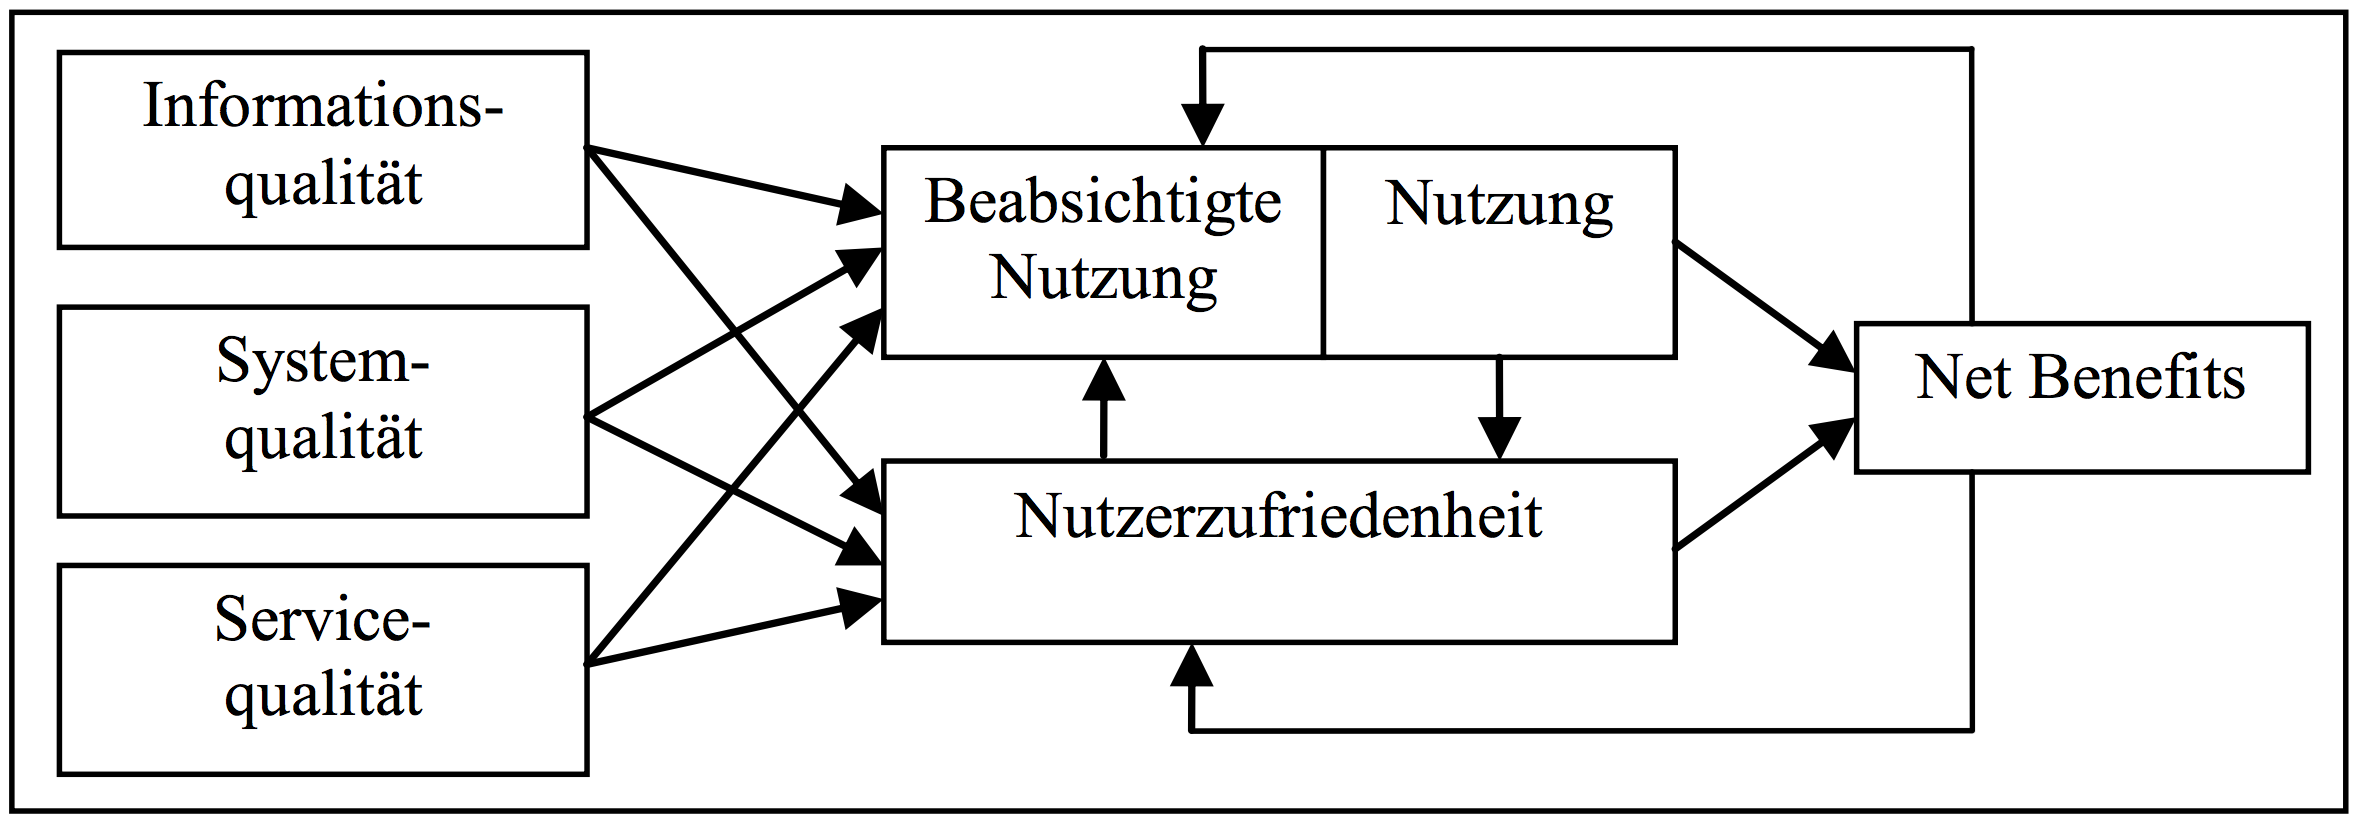
\includegraphics[width=1\textwidth]{Grafiken/issuccess.png}

Das im Rahmen dieses Papers verwendete IS Success Modell beinhaltet allerdings nur 4 Konstrukte, da erstens die Anzahl der Fragen streng reglementiert war und darüber hinaus auch nur eine geringe Response Rate erwartet wurde. Somit ist es mit dem kleinen sample besser möglich, qualitativ gute Aussagen zu treffen. Die Konstrukte sind in Tabelle XX \ref{tab:Forschungsmodell} genau definiert. Aufgrund der internationalen Ausrichtung des Kurses wurden die Fragen in Englisch gestellt, wobei eine Seven-point Likert Skala verwendet wurde. Die Antwortmöglichkeiten reichten von "`Strongly disagree (1)"' bis "`Strongly Agree (7)"'. Wie eingehend schon erwähnt, fand die Erhebung der Daten zu drei unterschiedlichen Zeitpunkten statt: zu Beginn des Kurses (T1), während des Kurses (T2) und zum Ende des Kurses (T3). Die Beantwortung der Umfrage unterlag einer freiwilligen Basis. Die im Forschungsmodell beschriebenen Items sind in den Fragebögen T2 und T3 enthalten. \todo{ITEM Enriched knowledge genau benennen}.
Für die Erstellung des Modells konnten jedoch nur Daten aus T2 und T3 verwendet werden, da die Teilnehmer zu Beginn des Kurses keine Angaben über ihren persönlichen Erfolg machen konnten (Frageitem: Enriched Knowledge fehlt in T1). 
 
% Tabellenformat 2

\begin{table}[ht] 
\footnotesize
\caption{Forschungsmodell}
\label{tab:Forschungsmodell} 
\begin{tabular}{@{}lp{10cm}r@{}} \toprule

\textbf{Konstrukt} & \textbf{Item} & \textbf{Factorloadings} \\ \midrule

Servicequalität & The Leuphana Digital School provides a proper level of online assistance and explanation & 0.8\\ 
& The teaching staff is highly availability for consultation & 0.7 \\
& The teaching staff provides satisfactory support to users using Leuphana Digital School & 0.6 \\ 
Systemqualität & Leuphana Digital School’s technical system has attractive features to appeal to the users. & 0.8\\ 
& Leuphana Digital School’s technical system is easy to use. & 0.7 \\
& Leuphana Digital School’s technical system provides a personalized information presentation. & 0.6 \\ 
Nutzerzufriedenheit & Most of the users bring a positive attitude or evaluation towards Leuphana Digital School. & 0.8\\ 
& Leuphana Digital School’s technical system is easy to use. & 0.7 \\ 
Persönlicher Nutzen & Leuphana Digital School helps you think through problems.  & 1\\ 
& All in all, my knowledge has been enriched as a result of the course & 0.4 \\ \addlinespace 
  \bottomrule

\end{tabular}	
\end{table}


% Tabellenformat 2

\begin{table}[ht] 
\caption{Forschungsmodell2}
\label{tab:Forschungsmodell} 
\begin{tabular}{@{}lp{12cm}r@{}} \toprule

\textbf{Konstrukt} & \textbf{Item} \\ \midrule

Servicequalität & The Leuphana Digital School provides a proper level of online assistance and explanation \\ \addlinespace
& The teaching staff is highly availability for consultation\\\addlinespace
& \parbox[t]{12cm}{The teaching staff provides satisfactory support to users using Leuphana Digital School} \\ \addlinespace
Systemqualität & \parbox[t]{12cm}{Leuphana Digital School’s technical system has attractive features to appeal to the users.}\\ \addlinespace
& Leuphana Digital School’s technical system is easy to use. \\\addlinespace
& \parbox[t]{12cm}{Leuphana Digital School’s technical system provides a personalized information presentation.} \\ \addlinespace
Nutzerzufriedenheit & \parbox[t]{12cm}{Most of the users bring a positive attitude or evaluation towards Leuphana Digital School.} \\ \addlinespace
& Leuphana Digital School’s technical system is easy to use.  \\ \addlinespace 
Persönlicher Nutzen & \parbox[t]{12cm}{Leuphana Digital School helps you think through problems.} \\ \addlinespace 
& \parbox[t]{12cm}{All in all, my knowledge has been enriched as a result of the course (nur in Fragebogen 2 und 3)} \\ \addlinespace 
  \bottomrule

\end{tabular}	
\end{table}

Teilnehmer
Die vorliegenden Daten entstammen aus Befragungen der Teilnehmer des MOOCs (Mentored Open Online Course) Psychology of Negotiations - Reaching Sustainable Agreements in Negotiations on "Commons"  der Leuphana Digital School. Der Kurs fand von Mai bis August 2014 statt und war offen für Teilnehmer aus der ganzen Welt. Die Teilnehmerzahl wurde auf 1000 begrenzt um die Qualität der Beratung und Führung durch Mentoren und Lehrende zu gewährleisten. Der Kurs war gebührenfrei. Bei erfolgreichem Abschluss konnten   Teilnehmer - gegen eine Gebühr von 20 	\texteuro - ein Zertifikat der Universität erhalten und 5 Credit Points (ECTS) zugeschrieben bekommen, welche dem eigenen Studium angerechnet werden konnten.   
Die Fragebögen wurden an alle Teilnehmer verschickt. Da die Anzahl der Kursteilnehmer, die den Fragebogen erhalten haben unbekannt ist, kann die Returnquote nicht angegeben werden. Gemessen an den Antworten, ist diese jedoch eher gering - vor allem in T2 und T3. Bei Ersterem lagen 32 Antworten vor, wovon nach Bereinigung von ungültigen oder unvollständigen Antworten 29 verwertbare waren. Die Bereinigung ungültiger und unvollständiger Antworten reduzierte die nutzbaren Antworten in T3 von 48 auf 36. Insgesamt liegen damit 65 Datensätze für die Modellüberprüfung vor, was einen relativ kleinen Stichprobenumfang darstellt. \cite[S. 5]{jakobowicz2006understanding} gaben an, dass für ein komplexes Modell ein Stichprobenumfang von mindestens 200 empfehlenswert ist, da ein geringer Stichprobenumfang zu Verzerrungen bei der Parameterschätzung und einem großem Standardfehler führen. Das in dieser Arbeit überprüfte Modell ist mit zwei unabhängig latenten (Systemqualität und Servicequalität) und zwei abhängig latenten Variablen (Nutzerzufriedenheit und Persönlicher Nutzen) verhältnismäßig einfach, daher kann auch ein kleiner Stichprobenumfang ausreichend Erkenntnisse liefern, gleichzeitig sollte bei der Interpretation der Ergebnisse jedoch der Stichprobenumfang berücksichtigt werden. 
Die Demographischen Daten der Fragebögen T2 und T3 lassen sich aus Tabelle\,\ref{tab:Demographische Daten} entnehmen. 
 

\begin{table}[ht] 
\caption{Demographische Daten}
\label{tab:Demographische Daten} 
\begin{tabular}{@{}lp{5cm}r@{}} \toprule

 & \textbf{Anzahl}&\textbf{in Prozent} \\ \midrule

\textit{Geschlecht}		& 				& \\ 
weiblich 				&  40 			& 62 \\
männlich				&  25			& 38 \\ 
Total					&  65			& 100 \\
\textit{Alter}			& 				&   \\
21-30 Jahre				&  35			& 54 \\
31-40 Jahre				&  10			& 15	  \\
> 41 Jahre				&  20 			& 31 \\
Total 					&  65			& 100 \\
\textit{Herkunft}		&				&   \\
Deutschland				& 27 			& 42  \\
Europa (excl. Deutschland) &18			& 28  \\
Afrika 					& 6				& 9   \\
Asien 					& 6				& 9   \\
Nordamerika				& 4				& 6   \\
Südamerika				& 4				& 6	 \\
Total					& 65				& 100  \\ 
  \bottomrule

\end{tabular}	
\end{table}


Data Analysis Technique
Instrument validation
We followed the procedures outlined by Gefen and Straub (2005) to test discriminant and convergent validity. Discriminant validity refers to whether the items measure the construct in question or other (related) constructs (Gefen and Straub, 2005). We verified discriminant validity using correlation matrix and factor analysis. Table 4 shows the correlation matrix with the square root of average variance extracted (AVE) values presented diagonally. The square root of the AVE value for the variables is consistently greater than the off-diagonal correlation values, suggesting satisfactory discriminant validity between the variables (Fornell and Larcker, 1981)

Zur Analyse im Rahmen dieser Arbeit wurde auf Strukturgleichungsmodellierung zurückgegriffen, 
For this paper, structural equation modeling (SEM) using partial least squares (PLS) was used to evaluate the research model and hypotheses.



